
%
% # INTRODUCTION:
%
% This write up is for Lab3: Logic Implementation Using IC's
%
% Specifically this was used for the class Logic Design Fundamentals (EECE 144)
% taught by Kurtis Kredo [http://www.ecst.csuchico.edu/~kkredo/]
% during the Fall 2011 semester at CSU Chico [www.csuchico.edu].
% 
% ## LaTeX
%
% This file is written for LaTeX [http://www.latex-project.org/]
% which is used to process this file in to a completely formatted
% document.
%
% If you are unfamiliar with LaTeX it can seem daunting at first
% (as with anything new) but there are many benefits.
% Imagine writing a document in Word except without
% having to worry about the tedious things such as line breaks,
% indentation, table of contents, appendices, font styles,
% heading sizes, citations/references, page numbers.
% LaTeX lets you focus on the content without
% worrying about the tedious details.  It is also excellent for
% producing mathematical formulas.
% 
% If you are collaborating with someone else you can simply edit
% the sections and paragraphs in this file as needed.
%
% To process this file use a command such as 'rubber'.
%
%   bash$ rubber skel.tex
%   (output to skel.dvi)
%   bash% rubber --pdf skel.tex
%   (output to skel.pdf)
%
% # AUTHORS (of this template):
%
%   Jeremiah Mahler <jmmahler@gmail.com>
%   https://www.google.com/profiles/jmmahler#about 
%
% # COPYRIGHT:
%
%   Copyright (C)  2011 Jeremiah Mahler <jmmahler@gmail.com>.
%   Permission is granted to copy, distribute and/or modify this document
%   under the terms of the GNU Free Documentation License, Version 1.3
%   or any later version published by the Free Software Foundation;
%   with no Invariant Sections, no Front-Cover Texts, and no Back-Cover Texts.
%   A copy of the license is included in the file "fdl-1.3.txt".
%

\documentclass[12pt]{article}
%\documentclass[10pt]{article}

%\usepackage{mslapa}
\usepackage{hyperref}
\usepackage{amsmath}
\usepackage{graphicx}
\usepackage{ulem}
%\usepackage{vmargin}
\usepackage{tabularx}
\usepackage{sectsty}
\usepackage{pbox}
\usepackage{bigstrut}
\usepackage{enumerate}
\usepackage{parskip}  % add spaces between paragraphs

%\usepackage{cleveref}

%\setpapersize{USletter}
\sectionfont{\normalsize}
\subsectionfont{\normalsize}

% configure \bigstrut size
% This configures spacing above and below rows in a tabularx.
%\renewcommand{\bigstrutjot}{6pt}
\renewcommand{\bigstrutjot}{2.0\jot}

\setlength{\parindent}{0in}

\raggedright

\begin{document}

% {{{ Cover Page

\centerline{\bf EECE 144}
\centerline{\bf Fall 2011}
\centerline{\bf}
\centerline{\bf Lab Report \#3}
\centerline{\bf Section 4}
\centerline{\bf 9/21/2011}

% signature area
\begin{center}
\begin{tabularx}{\textwidth}[b]{X l l}
Submitted by: & & \\
Signature & Printed Name & Date \\
\hline
\multicolumn{1}{|X|}{} & \multicolumn{1}{|l|}{\bigstrut \bf Jeremiah Mahler} & \multicolumn{1}{|l|}{\bf Sep 21, 2011} \\
\hline
\multicolumn{1}{|X|}{} & \multicolumn{1}{|l|}{\bigstrut \bf Marvanee Johnson} & \multicolumn{1}{|l|}{\bf Sep 21, 2011} \\
\hline
\end{tabularx}
\end{center}
% }}}

\section{Description/Objectives}

The objective of this lab is to build a working logic function
in hardware along with basic interfacing circuits using switches
and LEDs.

\section{Procedure}

\label{sec:plan}
Equation \ref{eq:fn1} will be used as the logic function to be implemented in
this lab.

\begin{align}
& a c + a' b + a b' c' \label{eq:fn1}
\end{align}

Before wiring the hardware it is a good idea to devise a plan using
a truth table and a diagram of the necessary gates.
The diagram built in Logisim should look similar to Figure \ref{fig:logisim1}.
The truth table (Figure \ref{fig:out1}) can be built by manually calculating
the output of the function or by using the Logisim simulation.
It is recommended to use both of these methods as this serves as a sanity
check for your calculations.
This check does not guarantee that they are both correct but it is unlikely that
they would both be wrong in exactly the same way.
\nocite{roth2009fundamentals}
\nocite{LOGISIM}

\begin{figure}[!hbt]

\center

\begin{tabular}[t]{| l | l | l | l |}
\hline
\multicolumn{4}{| c |}{$a c + a' b + a b' c'$} \\
\hline
$a$ & $b$ & $c$ & z (out) \\
\hline
0 & 0 & 0 & 0 \\
\hline
0 & 0 & 1 & 0 \\
\hline
0 & 1 & 0 & 1 \\
\hline
0 & 1 & 1 & 1 \\
\hline
1 & 0 & 0 & 1 \\
\hline
1 & 0 & 1 & 1 \\
\hline
1 & 1 & 0 & 0 \\
\hline
1 & 1 & 1 & 1 \\
\hline
\end{tabular}

\caption{Truth table of outputs for the function $a c + a' b + a b' c'$.}
\label{fig:out1}
\end{figure}

\begin{figure}[!hbtp]
\center
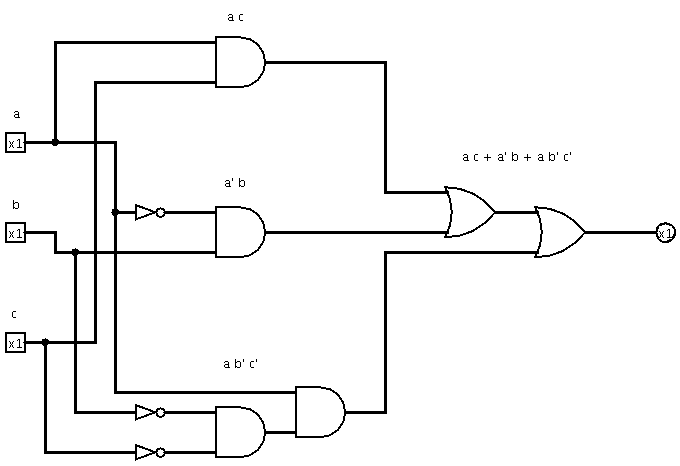
\includegraphics[scale=0.5]{Lab3-circuit}
\caption{Logic circuit $a c + a' b + a b' c'$ defined in Logisim.}
\label{fig:logisim1}
\end{figure}

\clearpage

\subsection{Interface Circuitry}

After the plan has been devised the next step is to implement the
function in hardware.

% input circuit
In order to provide hi/lo signals in to the 7400 series chips
\cite{wiki:7400_series} it is necessary to provide approximately 5 volts for
hi and 0 volts for low.
This can be done using a mechanical switch with one terminal connected
to a 5 volt source.
But when the switch opens to indicate 0 volts this open circuit condition
is indeterminate and is not guaranteed to be near 0 volts.
To remedy this situation a pull down resistor is used as show in Figure \ref{fig:pulldown}.
Any suitably large value for the resistor should work but it was found
that 1k worked whereas 10k did not.

\begin{figure}[!hbtp]
\center
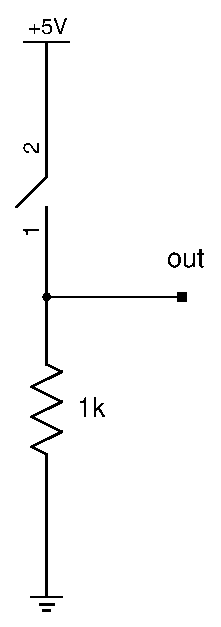
\includegraphics[scale=0.6]{pulldown}
\caption{Pull down resistor circuit.}
\label{fig:pulldown}
\end{figure}

% output circuit
To signal the final result of the logic circuit a LED will
be connected to the final output pin.
For the LEDs used in this lab the current should be approximately
20 mA.
If we assume that the diode behaves as a short circuit with
no voltage drop we can use Ohm's Law ($V = i \cdot R$) to calculate a
resistor value of 250 ohms ($5 / .020 = 250$).
Select a resistor with a value greater than or equal to this.
Also be aware that LEDs are directional and they will not illuminate
if they are backwards.

\subsection{Wiring}

The task of wiring the chips is tedious but it is nearly impossible
without a plan (see Section \ref{sec:plan}).

To wire the chips it is necessary to have all the pertinent data sheets.
These describe the function of each pin, the voltage characteristics and
the orientation of the pins.
The general procedure is as follows:
\begin{itemize}
	\item Choose a subset of the circuit to implement from Figure \ref{fig:logisim1}.
	\item Refer to the data sheet for the pin identification of the chip involved.
	\item Connect wires.
	\item Repeat until all subsets of the circuit have been implemented.
\end{itemize}

As an example, the diagram (Figure \ref{fig:logisim1}) showed that
each pin was connected to the NOT gates first.
So the first step was to connect each of the switches which represented
the inputs $a$, $b$, and $c$ to the corresponding pins on the 7404 NOT gate chip.

% testing
To test the output of a pin on a chip a voltmeter can be used.
The hi/low outputs will not be exactly 5 volts but they should be close
\footnote{Refer to the data sheet for the chip being used for the exact
threshold values.}.

%\clearpage

\section{Observations}

The output of the logic function should agree with the truth table
(Figure \ref{fig:out1}).

The voltage level outputs are unlikely to be exactly 0 volts and
5 volts for low and high.
During this lab it was found that a low
of 0.16 volts and a high of 4.68 volts was normal.

\clearpage
\section{Conclusion}

The construction of this logic circuit confirmed the expected behavior
as predicted through manual calculation and simulation.
The benefit of simulation and calculation was also shown by the
fact that wiring chips is tedious and time consuming.

% flush all the figures
%\clearpage

%\pagebreak
\renewcommand*{\refname}{\vspace{-8mm}}
\section{References}
%\bibliographystyle{plain}
%\bibliographystyle{mslapa}
\bibliographystyle{ieeetr}
\bibliography{../references}

% Appendix (if needed)

\end{document}

% vim:foldmethod=marker
